\documentclass[a4paper,11pt]{article}
\usepackage{latexsym}
\usepackage[dvipdfmx]{graphicx}
\usepackage{amsmath}
\usepackage{amssymb}
\usepackage{color}
\usepackage{listings}

\setlength{\textheight}{40\baselineskip}
\setlength{\topmargin}{35mm}
\addtolength{\topmargin}{-1.5in}

\setlength{\textwidth}{150mm}
\setlength{\oddsidemargin}{30mm}
\addtolength{\oddsidemargin}{-1in}
\setlength{\evensidemargin}{30mm}
\addtolength{\evensidemargin}{-1in}

\setlength{\footskip}{30mm}

\title{A Algorithm for Mapping Data to Storage Clusters}
\author{Kazuho Fujii}
\date{}

\begin{document}
\maketitle

\section{Introduction}

Mapping data to a storage cluster is a popular issue in distributed storage systems.
In other word, the issue is to decide which node should have the data.
Schemes of mapping data are required two characteristics.
One is distributing objects uniformly among the storage cluster.
This avoids bias of I/O requests to a specific node and the storage cluster gets efficient performance.
The other is suppressing data movement when the cluster is reorganized, e.g., adding a storage node by the reason that remaining capacity is small.

A simple solution is to put a centralized server that governs the position of data objects.
However, in this approach access clients should inquire to the master server about a node
that should have the read or written data.
The cost for this query is not negligible.

For solving this problem following approach is effective:
access clients and the storage cluster share a function that maps data objects to storage nodes.
The master server is not necessary in this approach.
Access clients can know a priori the storage node requested I/O.

Ceph\cite{ceph}, a popular distributed storage system, takes this approach.
The data mapping algorithm in Ceph is called CRUSH\cite{crush}.
It has some inner algorithms for mapping objects.
Straw bucket (or straw2, a new version of straw bucket) is the recommended algorithm.
It satisfies the required characteristics above.
It can map data objects uniformly and suppress data movement if the cluster is reorganized.
However, the calculation performance of straw bucket is the order of $O(N)$, where $N$ is the number of nodes.
Faster algorithms are required for enhancing the performance.

For this issue, I found a new bucket algorithm named {\it jump bucket}.
Its time complexity is $O((\log N)^2)$.
In this paper, I introduce the jump bucket algorithm.

\section{Related Work}

Other algorithms for mapping object than CRUSH are proposed. Especially, I am inspired by jump consistent hash\cite{jump-consistent-hash}. It is shown in Figure \ref{code_jumpconsistenthash}.
Its inputs are a 64 bit key and the number of items and its output is  an item number.
Note that the value of key in while loop is a 64 bit pseudo-random variable by a linear congruential generator\cite{lecuyer}.
The advantage of jump consistent hash is its calculation performance.
Its time complexity is $O(\log(N))$.
The remarkable idea in the algorithm is that it calculates only items where the object destination is change.
The detail is described in Section 3.

\begin{figure}[tbp]
\lstset{language=C}
\begin{footnotesize}
\begin{lstlisting}[frame=single]
int32_t jump_consistent_hash(uint64_t key, int32_t num_items) {
    uint64_t i = -1, j = 0;
    while (j < num_items) {
        i = j;
        key = key * 2862933555777941757ULL + 1;
        j = (i + 1) * ((double)(1LL << 31) / (double)((key >> 33) + 1));
    }
    return i;
}
\end{lstlisting}
\end{footnotesize}
\caption{Jump consistent hash algorithm in C.}
\label{code_jumpconsistenthash}
\end{figure}

The target situation of jump consistent hash is similar to list bucket. It is a inner algorithm of CRUSH.
Figure \ref{code_listbucket} shows an simple implementation of list bucket. Ceph use Jenkins' function\cite{jenkins} for the hash function.
Jump consistent hash and list bucket are suitable for circumstances in which the number of items is monotonically increased and never shrinks.
Jump consistent hash uses this restriction for getting good performance.
Thus, the idea in jump consistent hash is applicable for list bucket.

Unlike jump consistent hash, list bucket can weight items.
The third argument of Figure \ref{code_listbucket} is an array of sums of weights of items.
The $i$-th member of the array is the sum of items from the first item to the $i$-th item.
The probability where a item is chosen is in proportion to its weight.
Weighting items is required to CRUSH algorithm.
Hence, I extend jump consistent hash in order to enable it to weight items.

\begin{figure}[tbp]
\lstset{language=C}
\begin{footnotesize}
\begin{lstlisting}[frame=single]
int32_t list_bucket(uint64_t key, int32_t num_items, uint32_t *sum_weights) {
    int32_t i;
    for (i = num_items - 1; i > 0; i--) {
        uint64_t h = hash(key, i);
        h &= 0xffffffff;
        h *= sum_weights[i];
        h = h >> 32;
        if (h < sum_weights[i] - sum_weights[i - 1]) {
            break;
        }
    }
    return i;
}
\end{lstlisting}
\end{footnotesize}
\caption{List bucket algorithm in C.}
\label{code_listbucket}
\end{figure}


\section{Jump Bucket Algorithm}

Jump bucket algorithm maps a object having a key to an weighted item in bucket.
Figure \ref{code_jumpbucket} shows a C implementation of jump bucket.
The function is given a 64 bit key, the number of items and the array of the sums of item weights.
The length of the array of the sums of item weights is the number of items, $N$.
The $i$-th member of the array is the sum of items from the first item to the $i$-th item.
That is, the first member of the array is the weight of the first item and the last member of the array is the sum of all items.
The function returns a chosen item number in the range $[0, N)$.

\begin{figure}[tbp]
\lstset{language=C}
\begin{footnotesize}
\begin{lstlisting}[frame=single]
int32_t jump_bucket(uint64_t key, int32_t num_items, uint32_t *sum_weights) {
    int32_t i = 0;
    while (1) {
        uint32_t h = hash(i, key);
        h &= 0x7fffffff;
        double w = sum_weights[i]
            * ((double)(1UL << 31) / (double)(h + 1UL));
        if (w >= sum_weights[num_items - 1]) {
            break;
        }
        int32_t low = i;
        int32_t high = num_items;
        while (1) {
            int32_t middle = (low + high) / 2;
            if (sum_weights[middle] > w) {
                high = middle;
            } else {
                low = middle;
            }
            if (low + 1 == high) {
                i = low + 1;
                break;
            }
        }
    }
    return i;
}
\end{lstlisting}
\end{footnotesize}
\caption{Jump bucket algorithm in C.}
\label{code_jumpbucket}
\end{figure}

I summarize differences among jump bucket, jump consistent hash and list bucket in Table \ref{table_algorithms}.
Unlike jump consistent hash, we can specify weights to items in jump bucket.
The probability where a item is chosen is proportion to the weight of the item.
That is, the probability equals $w_i / \sum_{n=0}^{N-1} w_n$, where $w_i$ is the weight of the item $i$.
Note that the first item is $i=0$.
The differences between jump bucket and list bucket are speed and reorganization efficiency.
The former is described in Section 4 and Section 5 and the later is described in Section 6.

\begin{table}[tbp]
\begin{tabular}{|c|c|c|c|} \hline
& {\bf Jump Bucket} & {\bf List Bucket} & {\bf Jump Consistent Hash} \\\hline
{\bf Speed}           & $O((\log(N))^2)$ & $O(N)$      & $O(\log(N))$     \\\hline
{\bf Weighting Items} & available        & available   & unavailable     \\\hline
{\bf Adding Items}    & optimal          & optimal     & optimal          \\\hline
{\bf Changing Weight} &&& \\
{\bf of the Newest Item}& optimal & optimal & - \\\hline
{\bf Changing Weight} &&& \\
{\bf of Old Items}& poor & moderate & - \\\hline
\end{tabular}
\caption{Summary of characteristics of mapping algorithms.}
\label{table_algorithms}
\end{table}

Jump bucket algorithm use the key idea of jump consistent hash.
It is to calculate only items where its destination is changed.

Now I consider a case where add $(i+1)$-th item to a bucket already having $i$ items.
Suppose that the weight of $n$-th item is $w_n$.
The probability where the destination for a key is changed by adding the new item is
$w_{i+1} / \sum_{n=0}^{i+1} w_n$ if the bucket algorithm has the optimal reorganize performance.
The new destination is the new added item.
The probability the destination is not changed is $\sum_{n=0}^i w_n / \sum_{n=0}^{i+1} w_n$.
Therefore, when the $j$-th item ($j > i$) is added, the probability where the destination is not changed from the $i$-th addition is $\sum_{n=0}^i w_n / \sum_{n=0}^j w_n$.
Suppose that $r$ is a pseudo-random variable depending on the key and $i$.
And suppose that the destination is not changed when $j$-th item is added if and only if
\begin{equation}
r < \sum_{n=0}^i w_n \bigg/ \sum_{n=0}^j w_n. \label{jump_dist}
\end{equation}
With the largest $j$ satisfying eq. \eqref{jump_dist}, the $(j+1)$-th item is the next item where the destination for the key is changed, and the destination is the $(j+1)$-th item.
If there is no $j$ satisfying eq. \eqref{jump_dist}, the $i$-th item is the destination.

We can calculate the final destination by finding the next item where the destination is changed recursively until getting an item that has not the next. The first item is clearly 0.
The outer while loop in Figure \ref{code_jumpbucket} conducts this procedure.

I get a pseudo-random variable with a hash value by the item number and the key.
Unlike jump consistent hash, I get pseudo-random value with the current item number.
This is because I want get the same pseudo-random for the same item and the key for suppress unnecessary movement at reorganization.
The kind of the hash function is optional. I use Jenkins' function\cite{jenkins} here.
``(double)(h + 1LL) / (double)(1LL $<<$ 31)" in Figure \ref{code_jumpbucket} is a pseudo-random value between 0 and 1.

If ``w" in Figure \ref{code_jumpbucket} is larger than the sum of weights of all items, this means the destination change does not occur any more. The current destination is returned.

In order to search the next item satisfying eq. \eqref{jump_dist}, I use the binary search algorithm. The inner while loop is an implement of it.

\section{Performance Analysis}

The time complexity of jump bucket algorithm is determined by the product of the numbers of iterations of the inner while loop and the outer while loops.
The number of iterations of the outer while loop is $O(\log(N))$ because it is equivalent to jump consistent hash.
On the other hand, the time complexity of the inner loop is also $O(\log(N))$ because it is a binary search.
Therefore, the time complexity of jump bucket is $O((\log(N))^2)$. This is far smaller than the time complexity of list bucket $O(N)$.

\section{Performance Measurement}

I compare the calculation performance about three algorithms: list bucket, jump bucket and jump consistent hash.
The implementations are in Figure \ref{code_jumpconsistenthash}, Figure \ref{code_listbucket} and Figure \ref{code_jumpbucket}.
The source code was compiled on a 64-bit platform using Gnu C Compiler with -O2 option and measured on an CPU which model name is Intel(R) Celeron(R) 2980U @ 1.60GHz.

I measured mean execution time of each function for various keys. For comparing with jump consistent hash the weights of items equals each other.

Figure \ref{performance} shows the result. The performance of each algorithm get far different as number of items is larger.
The fastest algorithm is jump consistent hash, followed in order by jump bucket and list bucket.
Comparing jump bucket and list bucket, jump bucket is far faster then list bucket.

\begin{figure}[tbp]
  \begin{center}
    \includegraphics[width=80mm, angle=-90]{performance.eps}
  \end{center}
  \caption{Execution time of mapping algorithms.}
  \label{performance}
\end{figure}

\section{Reorganization}

I conducted experiments of objects movement under reorganization of buckets.
I tested five cases as following: adding a new item to the item list of the bucket, increasing weight of the last item in the item list, decreasing weight of the last item in the item list, increasing weight of the first item in the item list, decreasing weight of the first item in the item list. The first item of the item list represents the old items of the item list.

I choose items under various keys from a bucket that has five items and each item weight is unity.
I compare this object destination and new destination after the operation of the test case. In the cases of increasing item weight I change the weight to two, and in the cased of decreasing weight I change the weight to zero.

Figure \ref{reorganize} shows the result of the experiment.
Under the optimal behavior objcects do not move unnecessarily.
In the cases of adding a new item and operations to the last item weight, both of jump bucket and list bucket have optimum characteristic.
In the cases of changing the old item weight, two algorithm are different. Under list bucket objects movement is not optimal but moderate.
However, jump bucket gets a poor result.
Catastrophic movement occurs when the old item weight is changed.
This is because the changing of the first item's weight affects the next searched item.
It is disadvantage of jump bucket algorithm.
We must verify its effects under the operation.

\begin{figure}[tbp]
  \begin{center}
    \includegraphics[width=80mm, angle=-90]{reorganize.eps}
  \end{center}
  \caption{The percentage of objects moved under various reorganizations.}
  \label{reorganize}
\end{figure}

\section{Conclusion}

In this paper, I introduced a new bucket algorithm for CRUSH.
It is similar to list bucket algorithm, but its performance is far better than list bucket.
The disadvantage of the algorithm is that changing weight of an old item causes catastrophic data movements among items.
The algorithm can be suitable when the storage cluster grows monotonically.

\begin{thebibliography}{9}

\bibitem{ceph} S. A. Weil, S. A. Brandt, E. L. Miller, D. D. E. Long and C. Maltzahn. 2006.
Ceph: a scalable, high-performance distributed file system.
In {\it Proceedings of the 7th Symposium on Operating Systems Design and Implementation.}

\bibitem{crush} S. A. Weil, S. A. Brandt, E. L. Miller and C. Maltzahn. 2006.
CRUSH: controlled, scalable, decentralized placement of replicated data.
In {\it Proceedings of the 2006 ACM/IEEE Conference on
Supercomputing.}

\bibitem{jump-consistent-hash} J. Lamping and E. Veach. 2014.
A fast, minimal memory, consistent hash algorithm.
In {\it http://arxiv.org/pdf/1406.2294.pdf}\ .

\bibitem{lecuyer} P. L'Ecuyer. 1999.
Tables of linear congruential generators of different sizes and good lattice structure.
In {\it Mathematics of Computation 68 (225).}

\bibitem{jenkins} R. J. Jenkins. 1995-1997.
Hash functions for hash table lookup.
In {\it http://burtleburtle.net/bob/hash/evahash.html}\ .

\end{thebibliography}


\copyright\ 2016 \ KAZUHO FUJII

\end{document}
